% =============================================================================
% Episode 022: Key Statistics and Metrics
% Series: DIP-SMC-PSO Professional Toolkit
% Phase: 4 (Appendix & Reference)
% Duration: ~25 minutes | Pages: 10-12 | Complexity: Reference
% Dependencies: All previous phases (E001-E021)
% =============================================================================

% ==============================================================================
% MASTER TEMPLATE FOR PODCAST EPISODE CHEATSHEET PDFs
% ==============================================================================
% Purpose: Beginner-friendly, colorful, multi-page study guides (2-4 pages)
% Target Audience: Complete beginners (Path 0 learners)
% Visual Style: Infographic-style with vibrant colors, icons, callout boxes
% ==============================================================================

\documentclass[11pt,a4paper]{article}

% ------------------------------------------------------------------------------
% GEOMETRY & LAYOUT
% ------------------------------------------------------------------------------
\usepackage[top=1.5cm, bottom=1.5cm, left=1.5cm, right=1.5cm, headheight=14pt]{geometry}
\usepackage{multicol}
\usepackage{fancyhdr}
\pagestyle{fancy}

% ------------------------------------------------------------------------------
% COLOR PALETTE (Vibrant & Beginner-Friendly)
% ------------------------------------------------------------------------------
\usepackage{xcolor}
\definecolor{primary}{RGB}{41, 128, 185}      % Blue - Main concepts, headers
\definecolor{secondary}{RGB}{39, 174, 96}     % Green - Success, examples
\definecolor{accent}{RGB}{230, 126, 34}       % Orange - Important notes
\definecolor{warning}{RGB}{231, 76, 60}       % Red - Common pitfalls
\definecolor{background}{RGB}{236, 240, 241}  % Light gray - Callout boxes
\definecolor{codeblock}{RGB}{44, 62, 80}      % Dark blue-gray - Code background
\definecolor{highlight}{RGB}{241, 196, 15}    % Yellow - Highlights

% ------------------------------------------------------------------------------
% TIKZ & GRAPHICS
% ------------------------------------------------------------------------------
\usepackage{tikz}
\usetikzlibrary{shapes, arrows, positioning, calc, shadows, decorations.pathreplacing, backgrounds, fit}
\usepackage{graphicx}
\usepackage{float}

% TikZ styles for consistent diagrams
\tikzstyle{block} = [rectangle, draw, fill=primary!20, text width=5em, text centered, rounded corners, minimum height=3em, drop shadow]
\tikzstyle{arrow} = [thick,->,>=stealth]
\tikzstyle{process} = [rectangle, draw, fill=secondary!20, text width=6em, text centered, rounded corners, minimum height=3em]
\tikzstyle{decision} = [diamond, draw, fill=accent!20, text width=4.5em, text badly centered, inner sep=0pt]
\tikzstyle{cloud} = [ellipse, draw, fill=background, text width=5em, text centered, minimum height=2.5em]

% ------------------------------------------------------------------------------
% BOXES & CALLOUTS (tcolorbox)
% ------------------------------------------------------------------------------
\usepackage{tcolorbox}
\tcbuselibrary{skins, breakable, raster}

% Key Concept Box (Blue)
\newtcolorbox{keypoint}{
    enhanced,
    colback=primary!10,
    colframe=primary,
    fonttitle=\bfseries,
    title=\faLightbulb\ Key Concept,
    attach boxed title to top left={yshift=-2mm, xshift=5mm},
    boxed title style={colback=primary},
    breakable
}

% Example Box (Green)
\newtcolorbox{example}{
    enhanced,
    colback=secondary!10,
    colframe=secondary,
    fonttitle=\bfseries,
    title=\faCode\ Example,
    attach boxed title to top left={yshift=-2mm, xshift=5mm},
    boxed title style={colback=secondary},
    breakable
}

% Warning Box (Red)
\newtcolorbox{warning}{
    enhanced,
    colback=warning!10,
    colframe=warning,
    fonttitle=\bfseries,
    title=\faExclamationTriangle\ Common Pitfall,
    attach boxed title to top left={yshift=-2mm, xshift=5mm},
    boxed title style={colback=warning},
    breakable
}

% Tip Box (Orange)
\newtcolorbox{tip}{
    enhanced,
    colback=accent!10,
    colframe=accent,
    fonttitle=\bfseries,
    title=\faLightbulb\ Pro Tip,
    attach boxed title to top left={yshift=-2mm, xshift=5mm},
    boxed title style={colback=accent},
    breakable
}

% Summary Box (Light gray)
\newtcolorbox{summary}{
    enhanced,
    colback=background,
    colframe=codeblock,
    fonttitle=\bfseries,
    title=\faListUl\ Quick Summary,
    attach boxed title to top left={yshift=-2mm, xshift=5mm},
    boxed title style={colback=codeblock},
    breakable
}

% ------------------------------------------------------------------------------
% ICONS & SYMBOLS (fontawesome5)
% ------------------------------------------------------------------------------
\usepackage{fontawesome5}

% Custom icon commands for consistency
\newcommand{\iconKey}{\textcolor{primary}{\faLightbulb}}
\newcommand{\iconCode}{\textcolor{secondary}{\faCode}}
\newcommand{\iconWarning}{\textcolor{warning}{\faExclamationTriangle}}
\newcommand{\iconTip}{\textcolor{accent}{\faInfoCircle}}
\newcommand{\iconLink}{\textcolor{primary}{\faLink}}
\newcommand{\iconBook}{\textcolor{secondary}{\faBook}}
\newcommand{\iconTarget}{\textcolor{accent}{\faBullseye}}

% ------------------------------------------------------------------------------
% TYPOGRAPHY & FONTS
% ------------------------------------------------------------------------------
\usepackage{lmodern}
\usepackage[T1]{fontenc}
\usepackage[utf8]{inputenc}

% Section styling
\usepackage{titlesec}
\titleformat{\section}{\Large\bfseries\color{primary}}{\thesection}{1em}{}[\titlerule]
\titleformat{\subsection}{\large\bfseries\color{secondary}}{\thesubsection}{1em}{}

% ------------------------------------------------------------------------------
% CODE LISTINGS
% ------------------------------------------------------------------------------
\usepackage{listings}
\lstset{
    basicstyle=\ttfamily\footnotesize\color{white},
    backgroundcolor=\color{codeblock},
    keywordstyle=\color{primary!80},
    commentstyle=\color{secondary!60}\itshape,
    stringstyle=\color{accent!80},
    numbers=left,
    numberstyle=\tiny\color{white!50},
    stepnumber=1,
    numbersep=8pt,
    frame=single,
    rulecolor=\color{codeblock},
    breaklines=true,
    breakatwhitespace=true,
    tabsize=4,
    captionpos=b
}

% Python-specific styling
\lstdefinestyle{python}{
    language=Python,
    morekeywords={self, def, class, import, from, as, return, if, else, elif, for, while, True, False, None}
}

% YAML-specific styling
\lstdefinestyle{yaml}{
    basicstyle=\ttfamily\footnotesize,
    showstringspaces=false,
    commentstyle=\color{secondary!60}\itshape,
    keywordstyle=\color{primary!80}
}

% ------------------------------------------------------------------------------
% HYPERLINKS
% ------------------------------------------------------------------------------
\usepackage{hyperref}
\hypersetup{
    colorlinks=true,
    linkcolor=primary,
    urlcolor=secondary,
    citecolor=accent
}

% ------------------------------------------------------------------------------
% HEADER & FOOTER CUSTOMIZATION
% ------------------------------------------------------------------------------
\fancyhf{}
\fancyhead[L]{\textcolor{primary}{\textbf{DIP-SMC-PSO Podcast Cheatsheet}}}
\fancyhead[R]{\textcolor{secondary}{\episodetitle}}
\fancyfoot[C]{\textcolor{primary}{\thepage}}
\renewcommand{\headrulewidth}{0.5pt}
\renewcommand{\footrulewidth}{0.5pt}

% ------------------------------------------------------------------------------
% CUSTOM COMMANDS
% ------------------------------------------------------------------------------

% Episode title command (to be defined in each episode file)
\newcommand{\episodetitle}{Episode Title}

% Learning objective command
\newcommand{\learningobjective}[1]{%
    \begin{center}
    \begin{tcolorbox}[colback=highlight!30, colframe=accent, width=0.9\textwidth]
    \iconTarget\ \textbf{Learning Objective:} #1
    \end{tcolorbox}
    \end{center}
}

% Quick reference command (for formulas/code snippets)
\newcommand{\quickref}[2]{%
    \begin{tcolorbox}[colback=background, colframe=primary, title=\faBookmark\ #1]
    #2
    \end{tcolorbox}
}

% Resource link command
\newcommand{\resourcelink}[2]{%
    \iconLink\ \href{#1}{\textcolor{secondary}{#2}}
}

% ------------------------------------------------------------------------------
% TITLE PAGE FORMATTING
% ------------------------------------------------------------------------------
\usepackage{afterpage}

\newcommand{\makeepisodetitle}[4]{%
    \begin{titlepage}
    \begin{tikzpicture}[remember picture, overlay]
        % Background gradient
        \fill[primary!20] (current page.south west) rectangle (current page.north east);

        % Title box
        \node[
            fill=white,
            rounded corners=10pt,
            drop shadow,
            text width=0.8\paperwidth,
            align=center
        ] at (current page.center) {
            \Huge\bfseries\color{primary} #1 \\[1em]
            \Large\color{secondary} #2 \\[2em]
            \large\color{codeblock} Part #3 $\cdot$ Duration: #4 \\[1em]
            \normalsize\color{codeblock} \textit{Beginner-Friendly Visual Study Guide}
        };

        % Footer
        \node[
            anchor=south,
            text width=0.9\paperwidth,
            align=center
        ] at (current page.south) {
            \color{primary}\rule{0.8\paperwidth}{0.5pt} \\[0.5em]
            \small\color{codeblock}
            \textbf{Repository:} \url{https://github.com/theSadeQ/dip-smc-pso} \\
            \textbf{Documentation:} academic/paper/presentations/podcasts/episodes/ \\[1em]
        };
    \end{tikzpicture}
    \end{titlepage}
}

% ------------------------------------------------------------------------------
% MATH & EQUATIONS
% ------------------------------------------------------------------------------
\usepackage{amsmath, amssymb, amsthm}
\usepackage{mathtools}

% Equation box (highlighted equations)
\newcommand{\eqbox}[1]{%
    \begin{tcolorbox}[colback=primary!5, colframe=primary, boxrule=1pt]
    \begin{equation}
    #1
    \end{equation}
    \end{tcolorbox}
}

% ------------------------------------------------------------------------------
% TABLES
% ------------------------------------------------------------------------------
\usepackage{booktabs}
\usepackage{array}
\usepackage{multirow}
\usepackage{colortbl}

% Custom table colors
\newcommand{\tableheadcolor}{\rowcolor{primary!30}}

% ------------------------------------------------------------------------------
% END OF PREAMBLE
% ------------------------------------------------------------------------------


% Episode Metadata
\title{\textbf{E022: Key Statistics \& Metrics}}
\def\episodenumber{022}
\def\episodetitle{Key Statistics \& Metrics (Project Health Check)}
\def\episodecategory{Appendix \& Reference}
\def\difficulty{Reference}

\begin{document}
\makeepisodetitle

% =============================================================================
% SECTION 1: OVERVIEW
% =============================================================================
\section{Overview}

\subsection{What You'll Learn}
\begin{itemize}
  \item \textbf{Scale}: 105,000 lines of code, 358 Python files
  \item \textbf{Testing}: 4,563 tests (81\% unit, 15\% integration, 4\% system)
  \item \textbf{Performance}: Controllers at 23-62 microseconds (160-430x margin)
  \item \textbf{Production Readiness}: 23.9/100 (correct for research project)
\end{itemize}

\subsection{The Health Check Analogy}
\begin{highlightbox}
\textbf{Concept}: Like a doctor measures vital signs (heart rate, blood pressure), software projects have vital signs: Scale, Quality, Speed.

\textbf{Standard}: Every metric quoted is reproducible (clone repository, run commands, verify numbers).

\textbf{Mission}: Provide honest assessment without cherry-picking or rounding up.
\end{highlightbox}

% =============================================================================
% SECTION 2: VITAL SIGN 1 - SCALE
% =============================================================================
\section{Vital Sign 1: Scale}

\subsection{Headline Numbers}
\begin{center}
\begin{tabular}{lc}
\toprule
\textbf{Metric} & \textbf{Value} \\
\midrule
Total source lines & 105,000+ \\
Python files & 358 \\
Controllers & 15,000 lines (7 variants) \\
Dynamics/Plant & 12,000 lines (3 fidelity levels) \\
PSO Optimization & 18,000 lines \\
Utilities & 60,000 lines (40,000 in utils/) \\
\bottomrule
\end{tabular}
\end{center}

\subsection{Context: What 105,000 Lines Means}
\begin{itemize}
  \item \textbf{Comparison}: Boeing 737 fly-by-wire = 500,000 lines | Modern browser = 50 million
  \item \textbf{Category}: "Serious research tool" (not weekend script, not enterprise platform)
  \item \textbf{Novel Equivalent}: Similar to \emph{The Great Gatsby} (~100,000 characters)
\end{itemize}

\subsection{The Iceberg Principle}
\textbf{Rule}: For every 1 line of algorithm, need 6 lines of infrastructure.

\begin{itemize}
  \item \textbf{Algorithm (15\%)}: 15,000 lines (controllers + PSO core logic)
  \item \textbf{Infrastructure (85\%)}: 90,000 lines (validation, logging, monitoring, visualization)
\end{itemize}

\textbf{Why?} Making algorithms debuggable, verifiable, reproducible requires thousands of lines of supporting infrastructure.

\subsection{Infrastructure Breakdown}
\begin{itemize}
  \item \textbf{Configuration Validation}: Prevent physically impossible parameters (negative mass, imaginary damping)
  \item \textbf{Logging}: Capture every timestep with microsecond timestamps
  \item \textbf{Monitoring}: Detect deadline misses, constraint violations, numerical instabilities
  \item \textbf{Visualization}: Animations, performance curves, publication-quality figures
  \item \textbf{Analysis}: Confidence intervals, hypothesis tests, Monte Carlo aggregation
\end{itemize}

% =============================================================================
% SECTION 3: TEST SUITE - 4,563 CASES
% =============================================================================
\section{Test Suite: 4,563 Cases}

\subsection{Test Pyramid Distribution}
\begin{center}
\begin{tabular}{lccc}
\toprule
\textbf{Layer} & \textbf{Percentage} & \textbf{Count} & \textbf{Purpose} \\
\midrule
Unit Tests & 81\% & 3,678 & Isolated functions/methods \\
Integration Tests & 15\% & 681 & Components working together \\
System Tests & 4\% & 182 & End-to-end scenarios \\
\midrule
\textbf{Total} & \textbf{100\%} & \textbf{4,563} & \textbf{257 test files} \\
\bottomrule
\end{tabular}
\end{center}

\subsection{Execution Metrics}
\begin{itemize}
  \item \textbf{Runtime}: 45 seconds (all 4,563 tests)
  \item \textbf{Failures}: 0 (100\% pass rate)
  \item \textbf{Frequency}: Run after every commit (fast enough for zero friction)
\end{itemize}

\subsection{Coverage Campaign (Phase 4, Week 3)}
\begin{itemize}
  \item \textbf{Duration}: 16 sessions, 16.5 hours
  \item \textbf{Tests Added}: 668 new tests
  \item \textbf{Critical Modules}: 100\% coverage (10 modules including chattering detection, saturation, validators)
  \item \textbf{Overall Coverage}: 2.86\% (strategic completion: critical paths validated)
\end{itemize}

\subsection{Quality Over Quantity Example}
\textbf{Chattering Detection Algorithm}:
\begin{itemize}
  \item Module: 127 lines of code
  \item Tests: 47 (1 test per 2.7 lines)
  \item Coverage: 100\%
  \item Scenarios: Normal operation, high-frequency switching, edge cases (zero/constant control), numerical edge cases (inf/nan), extreme sampling rates
\end{itemize}

\textbf{Principle}: Validate critical behavior, not maximize coverage percentage.

% =============================================================================
% SECTION 4: CONTROLLER PERFORMANCE
% =============================================================================
\section{Controller Performance}

\subsection{Microsecond-Level Timings}
\begin{center}
\begin{tabular}{lcccc}
\toprule
\textbf{Controller} & \textbf{Time ($\mu$s)} & \textbf{Deadline} & \textbf{Margin} & \textbf{Budget Used} \\
\midrule
Classical SMC & 23 & 10,000 $\mu$s & 430x & 0.23\% \\
Super-Twisting & 31 & 10,000 $\mu$s & 322x & 0.31\% \\
Adaptive SMC & 45 & 10,000 $\mu$s & 222x & 0.45\% \\
Hybrid Adaptive STA & 62 & 10,000 $\mu$s & 161x & 0.62\% \\
\bottomrule
\end{tabular}
\end{center}

\textbf{Real-time Deadline}: 10ms (10,000 $\mu$s) for 100 Hz control loop

\subsection{Why Performance Margins Matter}
\begin{enumerate}
  \item \textbf{Jitter Tolerance}: Controllers using <1\% budget never miss deadlines (vs. 99\% usage with occasional misses)
  \item \textbf{Power Efficiency}: Finish computation quickly, sleep for remainder of cycle
  \item \textbf{Scalability}: Computational headroom for future features (sensor fusion, state estimation)
\end{enumerate}

\subsection{Marathon Analogy}
If 10ms deadline = marathon, controllers finish in first 100 meters, then wait at finish line.

\subsection{Complexity Cost}
Each layer of sophistication costs ~10-20 microseconds:
\begin{itemize}
  \item Classical SMC: Switching surface + sign function = 23 $\mu$s (baseline)
  \item Super-Twisting: + Differentiator + Integrator = +8 $\mu$s
  \item Adaptive SMC: + Dynamic gain adjustment = +14 $\mu$s
  \item Hybrid: + All sophistications = +17 $\mu$s
\end{itemize}

\subsection{Monitoring & Safety}
\begin{itemize}
  \item \textbf{Timeout}: 5ms per controller (half the step period)
  \item \textbf{Deadline Miss}: Logged if exceeded
  \item \textbf{Violation}: After 3 consecutive misses, weakly-hard constraint violation flagged
  \item \textbf{Principle}: Timing is a safety property, not performance optimization
\end{itemize}

% =============================================================================
% SECTION 5: SIMULATION SPEED
% =============================================================================
\section{Simulation Speed}

\subsection{Optimization Levels}
\begin{center}
\begin{tabular}{lcc}
\toprule
\textbf{Configuration} & \textbf{Time} & \textbf{Speedup} \\
\midrule
Pure Python (single sim) & 2.5s & 1.0x (baseline) \\
Numba JIT (single sim) & 0.8s & 3.1x \\
Vectorized batch (100 sims) & 12s total (8ms each) & 20.8x \\
Monte Carlo (1,000 sims) & 95s total & 26.3x \\
\bottomrule
\end{tabular}
\end{center}

\subsection{Researcher Impact}
\textbf{Use Case}: 500 Monte Carlo trials for confidence intervals

\begin{itemize}
  \item \textbf{Sequential Python}: 20 minutes (lunch break)
  \item \textbf{Vectorized Numba}: 45 seconds (immediate iteration)
\end{itemize}

\textbf{Principle}: Performance in research software reduces iteration cycle, enabling more hypotheses explored per working day.

\subsection{Benchmark Methodology}
\begin{itemize}
  \item \textbf{Timer}: Python \texttt{perf\_counter} (monotonic clock)
  \item \textbf{Iterations}: 1,000 runs per benchmark
  \item \textbf{Warm-up}: Discard first 100 iterations (JIT compilation, cache population)
  \item \textbf{Metric}: Median of remaining 900 iterations (robust against outliers)
  \item \textbf{Worst-Case}: Report 95th percentile for tail latency
\end{itemize}

\subsection{Reproducibility}
\begin{itemize}
  \item \textbf{Absolute Timings}: Vary by hardware (processor, memory, Python version)
  \item \textbf{Relative Ordering}: Should be consistent (Classical < STA < Adaptive < Hybrid)
  \item \textbf{Ratios}: STA ~1.3-1.5x slower than Classical (not 10x)
  \item \textbf{Validation}: Benchmark script checks ratios within expected ranges (green/yellow/red)
\end{itemize}

% =============================================================================
% SECTION 6: PSO OPTIMIZATION
% =============================================================================
\section{PSO Optimization}

\subsection{Default Configuration}
\begin{itemize}
  \item \textbf{Particles}: 50
  \item \textbf{Iterations}: 100
  \item \textbf{Total Simulations}: 5,000 (50 particles $\times$ 100 iterations)
\end{itemize}

\subsection{Runtime}
\begin{center}
\begin{tabular}{lcc}
\toprule
\textbf{Configuration} & \textbf{Runtime} & \textbf{Speedup} \\
\midrule
Single-threaded & 8 minutes & 1.0x \\
4-core parallel & 3 minutes & 2.8x \\
\bottomrule
\end{tabular}
\end{center}

\textbf{Note}: Not perfectly linear (2.8x vs. 4.0x) due to inter-particle communication overhead.

\subsection{Memory Footprint}
\begin{itemize}
  \item \textbf{Peak Memory}: 105 MB during PSO run
  \item \textbf{PSO Overhead}: ~20 MB (swarm tracking: positions, velocities, bests)
  \item \textbf{Context}: <1\% of modern laptop RAM (16 GB)
  \item \textbf{Benefit}: Run multiple optimization campaigns simultaneously without memory pressure
\end{itemize}

% =============================================================================
% SECTION 7: MEMORY MANAGEMENT
% =============================================================================
\section{Memory Management}

\subsection{10,000 Simulation Test}
\begin{itemize}
  \item \textbf{Initial Memory}: 85 MB
  \item \textbf{Final Memory (after 10K runs)}: 92 MB
  \item \textbf{Growth}: 7 MB total (8.2\%)
  \item \textbf{Threshold}: 10\% (PASS with margin)
  \item \textbf{Growth Rate}: 0.0 KB/hour
\end{itemize}

\subsection{Memory Management Mechanisms}
\begin{enumerate}
  \item \textbf{Bounded Deques}: History buffers with max length (old entries auto-discarded)
  \item \textbf{Explicit Cleanup}: Every controller has cleanup() method
  \item \textbf{Periodic GC}: Garbage collection at defined intervals
  \item \textbf{Weakref Patterns}: Prevent circular references (Episode 17)
\end{enumerate}

\subsection{Per-Controller Memory Usage}
\begin{center}
\begin{tabular}{lcc}
\toprule
\textbf{Controller} & \textbf{Memory (KB)} & \textbf{Growth Rate (KB/hr)} \\
\midrule
Classical SMC & 52 & 0.0 \\
Super-Twisting & 68 & 0.0 \\
Adaptive SMC & 91 & 0.0 \\
Hybrid Adaptive STA & 118 & 0.0 \\
\bottomrule
\end{tabular}
\end{center}

\textbf{Principle}: More complex controllers maintain more state, but all <1 MB and zero growth over time.

% =============================================================================
% SECTION 8: THREAD SAFETY
% =============================================================================
\section{Thread Safety}

\subsection{Validation Results}
\begin{itemize}
  \item \textbf{Tests}: 11 dedicated thread safety tests
  \item \textbf{Pass Rate}: 100\% (all 11 passing)
  \item \textbf{Race Conditions}: Zero detected
\end{itemize}

\subsection{Test Scenarios}
\begin{enumerate}
  \item Concurrent controller instantiation (multiple threads calling factory)
  \item Parallel execution of independent simulations
  \item Shared configuration access from multiple threads
\end{enumerate}

\subsection{Reproducibility}
\begin{itemize}
  \item \textbf{Bit-Identical Results}: Single-threaded vs. multi-threaded agree to $1 \times 10^{-10}$ (one ten-billionth)
  \item \textbf{Principle}: Controllers are pure functions (same inputs -> same outputs, no hidden mutable state)
\end{itemize}

% =============================================================================
% SECTION 9: DOCUMENTATION
% =============================================================================
\section{Documentation}

\subsection{Scale}
\begin{itemize}
  \item \textbf{Total Files}: 985 documentation files
  \item \textbf{Navigation Systems}: 11 independent systems
  \item \textbf{Category Indexes}: 43 across all domains
  \item \textbf{Learning Paths}: 5 (Path 0: 125-150 hrs -> Path 4: 12 hrs)
\end{itemize}

\subsection{Quality Control}
\begin{itemize}
  \item \textbf{Automated Checks}: Scan for broken links, missing code examples, AI-ish patterns
  \item \textbf{Flagged Files}: 12 out of 985
  \item \textbf{Pass Rate}: 98.8\%
\end{itemize}

\subsection{Documentation Standards (CLAUDE.md Section 18)}
\begin{itemize}
  \item \textbf{Direct}, not conversational
  \item \textbf{Specific}, not generic
  \item \textbf{Technical}, not marketing
\end{itemize}

\textbf{Exception}: Podcast episodes deliberately conversational (medium-appropriate).

% =============================================================================
% SECTION 10: RESEARCH DELIVERABLES
% =============================================================================
\section{Research Deliverables}

\subsection{Phase 5 Scorecard}
\begin{center}
\begin{tabular}{lc}
\toprule
\textbf{Category} & \textbf{Completion} \\
\midrule
Quick Wins (QW-1 to QW-5) & 5/5 (100\%) \\
Medium-Term (MT-5 to MT-8) & 4/4 (100\%) \\
Long-Term (LT-4, LT-6, LT-7) & 3/3 (100\%) \\
\midrule
\textbf{Total} & \textbf{11/11 (100\%)} \\
\bottomrule
\end{tabular}
\end{center}

\subsection{LT-7 Research Paper (Submission-Ready v2.1)}
\begin{itemize}
  \item \textbf{Figures}: 14 publication-quality (comparative performance, boundary layer optimization, Lyapunov analysis)
  \item \textbf{Bibliography}: 39 entries (12 foundational, 15 modern control theory, 12 software dependencies)
  \item \textbf{Software Citations}: All 36 dependencies formally cited (NumPy, SciPy, PySwarms, Numba, etc.)
  \item \textbf{Reproducibility Scripts}: Regenerate every figure from raw simulation data
\end{itemize}

% =============================================================================
% SECTION 11: PRODUCTION READINESS
% =============================================================================
\section{Production Readiness: 23.9/100}

\subsection{Why 23.9 Is the Correct Score}
\textbf{Context}: Research project not intended for production deployment.

\subsection{Quality Gates (8 Total)}
\begin{center}
\begin{tabular}{lc}
\toprule
\textbf{Gate} & \textbf{Status} \\
\midrule
Documentation Quality & 100/100 (PASS) \\
Test Pass Rate & 100\% (PASS) \\
Thread Safety & Validated (PASS) \\
Memory Management & Validated (PASS) \\
Controller Performance & 160-430x margin (PASS) \\
Research Quality & Paper submission-ready (PASS) \\
\textbf{Test Coverage} & \textbf{2.86\% (FAIL)} \\
\textbf{Formal Verification} & \textbf{Not completed (FAIL)} \\
\bottomrule
\end{tabular}
\end{center}

\textbf{Result}: 6/8 gates passing (7/8 if research quality counted separately)

\subsection{Production vs. Research Quality}
\begin{center}
\begin{tabular}{lc}
\toprule
\textbf{System Type} & \textbf{Target Score} \\
\midrule
Safety-critical (medical, aircraft) & 90+ \\
Commercial software & 70-80 \\
Open-source development tools & 60-70 \\
Research prototypes (validated algorithms) & 20-30 \\
\bottomrule
\end{tabular}
\end{center}

\subsection{To Reach Production Readiness}
\textbf{Estimated Effort}: 200-300 hours

\begin{itemize}
  \item Formal verification (model checking, theorem proving)
  \item Fault injection testing (hardware failures, graceful degradation)
  \item Security auditing (web interface)
  \item PLC integration (real hardware)
  \item Safety certification
\end{itemize}

\textbf{Status}: Deferred until post-publication (Phase 6-7 future work).

% =============================================================================
% SECTION 12: KEY TAKEAWAYS
% =============================================================================
\section{Key Takeaways}

\subsection{Reproducible Metrics}
\begin{itemize}
  \item 105,000 lines across 358 files
  \item 4,563 tests, 100\% pass rate
  \item Controllers: 23-62 $\mu$s (160-430x deadline margin)
  \item PSO: 5,000 simulations in 8 minutes
  \item Memory: 0.0 KB/hr growth over 10,000 simulations
  \item Documentation: 985 files, 98.8\% pass rate
  \item Research: 11/11 tasks complete
  \item Production: 23.9/100 (correct for research project)
\end{itemize}

\subsection{Verification Commands}
\begin{lstlisting}[style=bashstyle]
# Test counts and pass rates
python -m pytest tests/ --co -q

# Line count
wc -l src/**/*.py

# Memory validation
python -m pytest tests/test_integration/test_memory_management/ -v

# Benchmarks
cd benchmarks/ && python run_benchmarks.py
\end{lstlisting}

\subsection{The Fundamental Principle}
\begin{highlightbox}
\textbf{Research Software Standard}: Metrics without reproducibility are marketing. Metrics with reproducibility are science.

\textbf{Mission-Driven Development}: Metrics follow the mission, not the other way around. We measure what we built, we don't build to hit measurements.
\end{highlightbox}

% =============================================================================
% CHECKLIST: STATISTICS VERIFICATION
% =============================================================================
\section*{Checklist: Verify Project Statistics}

\begin{center}
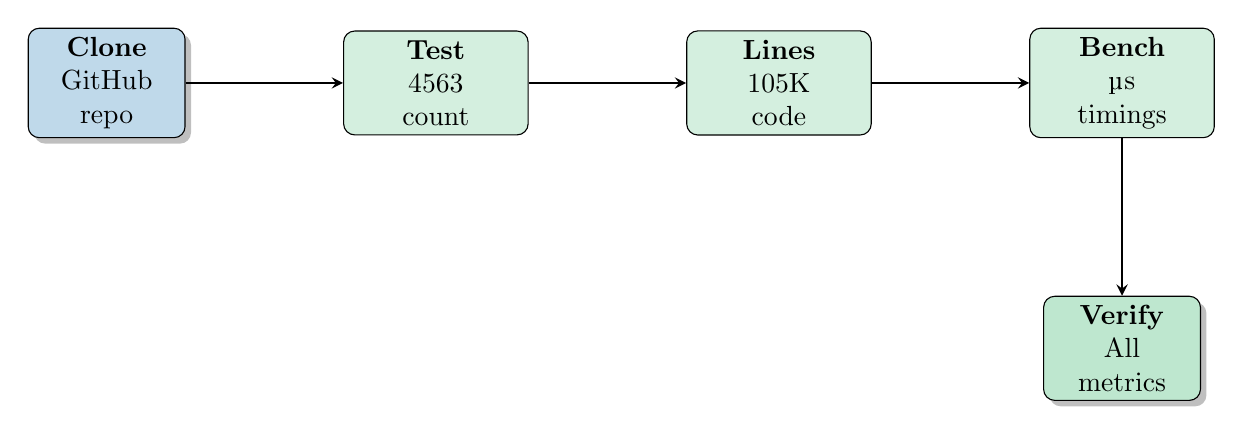
\begin{tikzpicture}[node distance=2cm]
    \node[block, fill=primary!30] (clone) {\textbf{Clone}\\GitHub\\repo};
    \node[process, right=of clone] (test) {\textbf{Test}\\4563\\count};
    \node[process, right=of test] (lines) {\textbf{Lines}\\105K\\code};
    \node[process, right=of lines] (bench) {\textbf{Bench}\\µs\\timings};
    \node[block, fill=secondary!30, below=of bench] (verify) {\textbf{Verify}\\All\\metrics};

    \draw[arrow] (clone) -- (test);
    \draw[arrow] (test) -- (lines);
    \draw[arrow] (lines) -- (bench);
    \draw[arrow] (bench) -- (verify);
\end{tikzpicture}
\end{center}

\begin{itemize}
  \item[$\square$] \textbf{Clone Repository}: \texttt{git clone https://github.com/theSadeQ/dip-smc-pso}
  \item[$\square$] \textbf{Test Count}: Run \texttt{pytest --co -q} (should show 4,563 tests)
  \item[$\square$] \textbf{Line Count}: Run \texttt{wc -l src/**/*.py} (should show ~105K lines)
  \item[$\square$] \textbf{Benchmarks}: Run benchmark scripts (verify microsecond timings)
  \item[$\square$] \textbf{Memory Test}: Run memory validation suite (verify 0.0 KB/hr growth)
  \item[$\square$] \textbf{Thread Safety}: Run thread safety tests (verify 11/11 passing)
  \item[$\square$] \textbf{Documentation}: Count files in \texttt{docs/} (should show ~985 files)
  \item[$\square$] \textbf{Research Paper}: Check \texttt{academic/paper/publications/} (LT-7 v2.1)
\end{itemize}

% =============================================================================
% NEXT STEPS
% =============================================================================
\section*{Next Steps}
\begin{itemize}
  \item \textbf{E023}: Visual diagrams and schematics (describing system architecture verbally)
  \item \textbf{E024}: Lessons learned and best practices (6-month development retrospective)
  \item \textbf{E025-E029}: Appendix reference (5-part deep dive into technical details)
\end{itemize}

\end{document}
